\section{Scheduler Configuration: Classes and Nodepools}
\label{sec:ducc.classes}

The class configuration file is used by the Resource Manager configure the rules used for job
scheduling. See the \hyperref[sec:]{Resource Manager chapter} for a detailed description of the DUCC
schedueler, scheduling classes, and how classes are used to configure the scheduling process.

The scheduler  configuration file is specified in ducc.properties. The default name is 
ducc.classes and is specified by the property {\em ducc.rm.class.definitions}.
  
\subsection{Nodepools}

\subsubsection{Overview}
    A {\em nodepool} is a grouping of a subset of the physical nodes to allow differing
    scheduling policies to be applied to different nodes in the system.  Some typical
    nodepool groupings might include:
    \begin{enumerate}
      \item Group Intel and Power nodes separately so that users may submit jobs that run
        only in Intel architecture, or only Power, or ``don't care''.
      \item Designate a group of nodes with large locally attached disks such that users
        can run jobs that require thos disks.
      \item Designate a specific set of nodes with specialized hardware such as high-speed
        network, such that jobs can be scheduled to run only on those nodes.
    \end{enumerate}

    A Nodepool is a subset of some larger collection of nodes.  Nodepools themselves may be
    further subdivided.  Nodepools may not overlap: every node belongs to one and exactly
    one nodepool.  During system start-up the consistency of nodepool definition is checked
    and the system will refuse to start if the configuration is incorrect.

    For example, the diagram below is an abstract representation of all the nodes in a
    system.  There are five nodepools defined:
    \begin{itemize}
      \item Nodepool ``Default'' is subdivided into three pools, NP1, NP2, and NP3.  All
        the nodes not contained in NP1, NP2, and NP3 belong to the pool called ``Default''.
      \item Nodepool NP1 is not further subdivided.
      \item Nodepool NP2 is not firther subdivided.
      \item Nodepool NP3 is further subdivided to form NP4.  All nodes within NP3 but
        not in NP4 are contained in NP3.
      \item Nodepool NP4 is not further subdivided.
    \end{itemize}

    \begin{figure}[H]
      \centering
      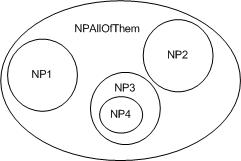
\includegraphics[bb=0 0 241 161, width=5.5in]{images/Nodepool1.jpg}
      \caption{Nodepool Example}
      \label{fig:Nodepools1}
    \end{figure}

    In the figure below the Nodepools are incorrectly defined for two reasons:
    \begin{enumerate}
       \item NP1 and NP2 overlap.
       \item NP4 overlaps both nodepool ``Default'' and NP3.
    \end{enumerate}
    
    \begin{figure}[H]
      \centering
      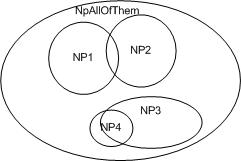
\includegraphics[bb=0 0 241 161, width=5.5in]{images/Nodepool2.jpg}
      \caption{Nodepools: Overlapping Pools are Incorrect}
      \label{fig:Nodepools2}
    \end{figure}

    Multiple ``top-level'' nodepools are allowed.  A ``top-level'' nodepool has no containing
    pool.  Multiple top-level pools logically divide a cluster of machines into {\em multiple
      independent clusters} from the standpoint of the scheduler.  Work scheduled over one
    pool in no way affects work scheduled over the other pool.  The figure below shows an
    abstract nodepool configuration with two top-level nodepools, ``Top-NP1'' and ``Top-NP2''.
    \begin{figure}[H]
      \centering
      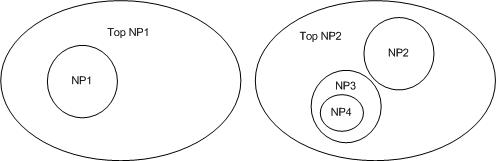
\includegraphics[bb=0 0 496 161, width=5.5in]{images/Nodepool3.jpg}
      \caption{Nodepools: Multiple top-level Nodepools}
      \label{fig:Nodepools3}
    \end{figure}

\subsubsection{Scheduling considerations}
    A primary goal of the scheduler is to insure that no resources are left idle if there
    is pending work that is able to use those resources.  Therefore, work scheduled to
    a class defined over a specific nodepool (say, NpAllOfThem), may be scheduled on nodes
    in any of the nodepools contained within NpAllOfThem.  If work defined over a
    subpool (such as NP1) arrives, processes on nodes in NP1 that were scheduled for
    NpAllOfThem are considered ``squatters'' and are the most likely candidates for
    eviction. (Processes assigned to their proper nodepools are considered ``residents''
    and are evicted only after all ``squatters'' have been evicted.)  The scheduler strives
    to avoid creating ``squatters''.

    Because non-preemptable process can't be preempeted, work submitted to a class
    implementing one of the non-preemptable policies (FIXED or RESERVE) are never allowed
    to ``squat'' in other nodepools and will scheduled only on the nodes in their
    proper nodepool.

    In the case of multiple top-level nodepools: these nodepools and their subpools
    form independent scheduling groups.  Specifically, fair-share allocations over any
    nodepool in one top-level pool does NOT affect the fair-share allocations for jobs
    in any other top-level nodepool.

\subsubsection{Configuration}
    DUCC uses a simplified JSON-like structure to define nodepools.

    At least one nodepool definition is required.  This nodepool need not have any subpools or node
    definitions.  The first top-level nodepool is considered the ``default'' nodepool.  A node not
    named specifically within one of the node files which checks in with DUCC is assigned to this
    first, or ``default'' nodepool. 

    Thus, if only one nodepool is defined with no other attributes, all nodes are
    assigned to that pool.

    A nodepool definition consists of the token ``Nodepool'' followed by its
    name, followed by a block delimeted with ``curly'' braces \{ and \}.  This
    block contains the attributes of the nodepool as key/value pairs.
    Lineneds are ignored.  A semicolon $;$ may optionally be used to
    delimit key/value pairs for readability, and an equals sign ``='' may optinally
    be used to delimit keys from values, also just for readability.

    The attributes of a Nodepool are:
    \begin{definition}
      \item[domain] This is valid only in the ``default'' nodepool.  Any node
        in any nodfile which does not have a doman, and any node which checks
        in with the schedule without a domain name is assigned this domain name
        in order that the scheduler may deal entirely with full-qualified node names.
      \item[nodefile] This is the name of a file containing the names of the nodes
        which are members of this nodepool.
      \item[parent] This is used to indicate which nodepool is the logical parent.
        Any nodepool without a ``parent'' is considered a top-level nodepool.
    \end{definition}
        
    The following example defines six nodepools, 
    \begin{enumerate}
      \item A top-level nodepool called ``--default--'',
      \item A top-level nodepool called ``jobdriver'',
      \item A subpool of ``--default--'' called ``intel'',
      \item A subpool of ``--default--'' called ``power'',
      \item A subpool of ``intel'' called ``nightly-test'',
      \item And a subpool of ``power'' called ``testing-p7'',
    \end{enumerate}
    
\begin{verbatim}
    Nodepool --default--  { domain bluej.net }
    Nodepool jobdriver    { nodefile jobdriver.nodes }
    
    Nodepool intel        { nodefile intel.nodes        ; parent --default-- }
    Nodepool power        { nodefile power.nodes        ; parent --default-- }

    Nodepool nightly-test { nodefile nightly-test.nodes ; parent intel }
    Nodepool timing-p7    { nodefile timing-p7.nodes    ; parent power }
\end{verbatim}
    
\subsection{Class Definitions}

    Scheduler classes are defined in the same simplified JSON-like language as
    nodepools.

    A simple inheritance (or ``template'') scheme is supported for classes.  Any
    class may be configured to ``derive'' from any other class.  In this case, the
    child class acquires all the attributes of the parent class, any of which may
    be selectively overridden.  Multiple inheritance is not supported but
    nested inheritance is; that is, class A may inherit from class B which inherits
    from class C and so on. In this way, generalized templates for the site's
    class structure may be defined.  

    The general form of a class definition consists of the keword Class, followed
    by the name of the class, and then optionally by the name of a ``parent'' class
    whose characteristics it inherits.   Following the name (and optionally parent class
    name) are the attributes of the class, also within a \{ \} block.

    The attributes defined for classes are:
    \begin{description}
      \item[abstract] If specified, this indicates this class is a template ONLY. It is used
        as a model for oher classes.  Values are ``true'' or ``false''.  The default is
        ``false''.
      \item[cap] This specifies the largest number of shares any job in this class
        may be assigned.  It may be an absolute number or a percentage.  If specified as
        a percentage (i.e. it contains a trailing \%), it specifies a percentage of the
        total nodes in the containing nodepool.
      \item[debug] FAIR_SHARE only. This specifies the name of a class to substitute
        for jobs submitted for debug.
      \item[expand-by-doubling] FAIR_SHARE only.  If ``true'', and the ``initialization-cap'' is
        set, then after any process has initialized, the job will expand to its maximum allowable
        shares by doubling in size each scheduling cycle.
      \item[initialization-cap] FAIR_SHARE only. If specified, this is the largest number of processes this job
        may be assigned until at least one process has successfully completed initialization.
      \item[max-processes] FIXED-SHARE only.  This is the largest number of FIXED-SHARE,
        non-preemptable shares any single job may be assigned.
      \item[prediction-fudge] FAIR_SHARE only. When the scheduler is considering expanding the
        number of processes for a job it tries to determine if the job may complete before those
        processes are allocated and initialized.  The ``prediction-fudge'' adds some amount of 
        time (in milliseconds) to the projected completion time.  This allows installations to
        prevent jobs from expanding when they were otherwise going to end in a few minutes
        anyway.
      \item[nodepool] If specified, jobs for this class are assigned to nodes in this nodepool. 
      \item[policy] This is the scheduling policy, one of FAIR_SHARE, FIXED_SHARE, or RESERVE. This
        attribute is required (there is no default).
      \item[priority] This is the scheduling priority for jobs in this class.
      \item[weight] FAIR_SHARE only. This is the fair-share weight for jobs in this class.
      
    \end{description}
    
